Given a graph $G=(V,E)$, a vertex cover is a subset $S \subseteq V$, so that for each edge $(u,v) \in E$ at least one of $u$ or $v$ lies in $S$.

Vertex cover decision problem (VC):
\begin{itemize} 
	\item Instance: graph $G$, integer $k$
	\item Question: does $G$ have a vertex cover of size at most $k$?
\end{itemize}

\subsection{Approximation Algorithm}
VC-OPT:
\begin{itemize}
	\item Instance: Graph $G$
	\item Goal: Find the size of the smallest vertex cover in $G$.
\end{itemize}

Exercise: Show how to finding the size of the vertex cover allows you to find the VC of that size.

Instance $I$ is just a graph. OPT($I$) = size of the subset VC in $I$. Let $A$ be any algorithm that find some vertex cover in a given instance $I$. Let $A(I)$ be the size of the vertex cover returned by $I$. If $A$ solve VC exactly then $A(I)$ = OPT($I$) $\forall I$. $A$ is a c-approximation algorithm if $\frac{A(I)}{OPT(I)} \le C, \forall I$. If $A$ is an exact optimization algorithm, then $c = 1$. Efficient algorithm $A$ may not achieve $c = 1$. We want $A$ that achieves a small approximation factor $\ge 1$.

Suppose we can lower bound the value of OPT($I$) for each $I$. Let $\ell (I) \le OPT(I) \forall I$. If we can prove that $\frac{A(I)}{\ell(I)} \le c$ for some $c$, then $\frac{A(I)}{OPT(I)} \le c$.

Given the following graph $I$, how to find the lower bound of OPT($I$).
\begin{figure}[H]
	\centering
	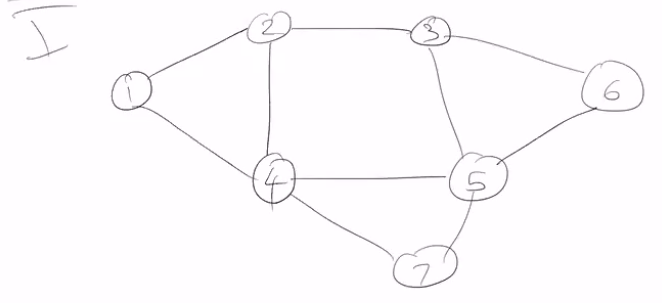
\includegraphics[width=0.5\textwidth]{fig/vc-low-bound.png}
\end{figure}

Matching is a set of edges that do not share any end point. The size of a matching is a lower bound on the size of a vertex cover. If on an instance $I$, we find a matching $M$, then the size VC $\ge |M|$. 

Note that maximal and maximum are two different concepts:
\begin{itemize}
	\item Maximal matching in a graph $I$ is a matching $M$ that cannot be extended. i.e, cannot add any edge to $M$ and still have a matching.
	\item Maximum matching is the matching set with the biggest set.
\end{itemize}

For example, in the following graph, red edges consist of a maximum matching while the green edge is a maximal matching by itself. It is because we are not able to expand any more after choosing the green edge. If we choose randomly, most of time we may end up with maximal matching instead of maximum. But maximal matching is actually enough for lower bound approximation.
\begin{figure}[H]
	\centering
	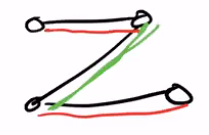
\includegraphics[width=0.3\textwidth]{fig/vc-max.png}
\end{figure}
Size of maximal matching is a lower bound on the size of the vertex cover. In the following example, black edges form a maximal matching.
\begin{figure}[H]
	\centering
	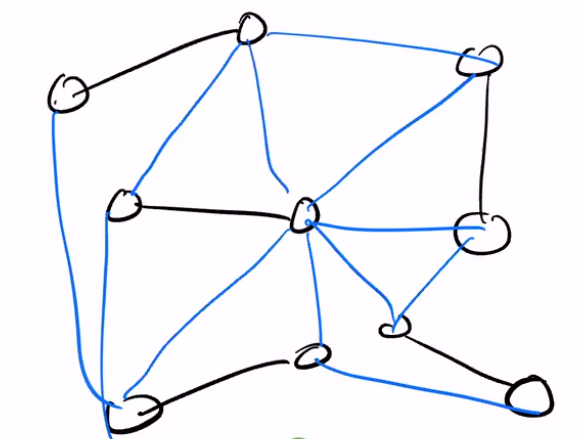
\includegraphics[width=0.3\textwidth]{fig/vc-matching.png}
\end{figure}

If $(u, v)$ is an edge that is not in the maximal matching, either $u$ or $v$ musts be an end point of some matching edge. In the opposite case, could you have an edge $(u, v)$, neither of whose end points has been matched into the maximal matching. The answer is no, since if such edge exist, we could actually add it into the maximal matching.

Find the vertex cover as follows: find a maximal matching $M = \{(u_1, v_1), (u_2, v_2) \cdots , (u_k, v_k)\}$. Pick all $2k$ vertices that are end points of edges in $M$. This is a vertex cover.

\subsection{Proof}
Suppose for contradiction, $\exists (u, v):$ neither $u$ nor $v$ $\in$ matching $M = \{u_1, u_2, \cdots, u_k, v_1, \cdots, v_k\}$. Then $(u, v)$ could have been added to $M$, contradicting the fact that $M$ is maximal.

Lower bound on the size of a vertex cover is $k$.

Our algorithm produces a C-approximation for $c = \frac{2k}{k} = 2$. 

Given graph $I$: how to find a maximal matching?  

A greedy algorithm works. Arrange edges in arbitrary order $e_1, e_2, \cdots, e_m$. $M = \emptyset$. For $i = 1$ to $m$, if $M \cup {e_i}$ is a matching, then $M = M \cup {e_i}$.

Could there be an edge $(u, v)$ in $I$ such that $M$ could be extended by $(u, v)$? The answer is NO. So $M$ is a maximal matching.

In conclusion, 2-approximation for VC given instance $I$:
\begin{itemize}
	\item find the maximal matching $M$
	\item output the set of of vertices consisting of both end points of each edge in $M$.
\end{itemize}























































